\hypertarget{kapitaal}{%
\chapter{Kapitaal}\label{kapitaal}}
\vspace{-1em}
\begin{blockquotebox}
    Overal waar we naar beschavingen kijken, treffen we een systeem aan dat op grote schaal in de toekomstige menselijke behoeften voorziet. Terwijl we nog onze winterkleding dragen om ons tegen de kou te beschermen, is de lente-collectie al onderweg naar de winkels. In de fabrieken worden ondertussen lichte stoffen geweven voor de kleding die we volgende zomer zullen dragen, en worden garens gesponnen voor de winterkleding van het jaar daarop. Wanneer we ziek worden, is de hulp van een arts noodzakelijk. Bij juridische conflicten is het advies van een advocaat onmisbaar. In dergelijke situaties zou het veel te laat zijn om op dat moment pas te beginnen met het verwerven van de benodigde medische of juridische kennis en vaardigheden, of om te proberen de gespecialiseerde opleiding van anderen te organiseren, zelfs als men over de benodigde middelen zou beschikken. In ontwikkelde landen worden de behoeften van de samenleving aan dergelijke diensten op tijd ingevuld door ervaren en deskundige professionals, die zich jaren van tevoren al op hun vakgebied hebben voorbereid en sindsdien uitgebreide praktijkervaring hebben opgedaan. Terwijl we zo profiteren van de vooruitziendheid uit het verleden, worden velen op onze universiteiten opgeleid om in de toekomst aan de behoeften van de samenleving te voldoen.\footnotemark
    \par\raggedleft--- Carl Menger\index{Carl Menger}
\end{blockquotebox}
\footautocite{58}


\lettrine{I}n het vorige hoofdstuk bespraken we het begrip eigendom in economische termen en de ontwikkeling van dit menselijke hulpmiddel in de loop van de tijd. De economische wetenschap maakt binnen alle vormen van eigendom een onderscheid tussen consumptiegoederen\index{consumptiegoed}, die eigendom zijn voor het nut dat ze hen bieden, en kapitaalgoederen\index{kapitaalgoederen}, die we bezitten omdat ze gebruikt kunnen worden om nuttige consumptiegoederen\index{consumptiegoed} te produceren. Kapitaalgoederen, ook goederen van hogere orde genoemd, zijn alle goederen die niet geconsumeerd worden, maar die worden gebruikt voor de productie\index{productie} van consumptiegoederen\index{consumptiegoed} of goederen van een lagere orde. Wat van een goed een consumptiegoed\index{consumptiegoed} of kapitaalgoed\index{kapitaalgoederen} maakt, is niet inherent aan het goed zelf, maar hangt af van hoe het goed gebruikt wordt door de persoon die het bezit. Hetzelfde goed kan gebruikt worden als kapitaalgoed\index{kapitaalgoederen} of als consumptiegoed\index{consumptiegoed}, afhankelijk van de context. Een computer die gebruikt wordt om films te kijken en op het web te surfen is een consumptiegoed\index{consumptiegoed}, maar dezelfde computer die gebruikt wordt om een boek te schrijven is een kapitaalgoed\index{kapitaalgoederen}. Een auto kan een kapitaalgoed\index{kapitaalgoederen} zijn als hij als taxi gebruikt wordt, maar een consumptiegoed\index{consumptiegoed} als hij puur voor recreatieve reizen gebruikt wordt. Maïskorrels kunnen een consumptiegoed\index{consumptiegoed} zijn als ze opgegeten worden, maar een kapitaalgoed\index{kapitaalgoederen} als ze geplant worden om meer maïs te verbouwen.

Dit hoofdstuk bespreekt het concept van kapitaal\index{kapitaal} op een abstracte manier. Na het introduceren van geld en de uitgebreide marktorde in de komende hoofdstukken, zal Hoofdstuk 12 kapitaal\index{kapitaal} behandelen in de context van een moderne monetaire economische orde. Deel IV van het boek zal de problemen bespreken van centrale planning op de kapitaalmarkten.

\hypertarget{verlenging-van-het-productieproces}{%
\section{Verlenging van het productieproces}\label{verlenging-van-het-productieproces}}

De invoering van kapitaal\index{kapitaal} in economische productie\index{productie} maakt een verlenging van de productieperiode noodzakelijk. Zonder kapitaalgoederen\index{kapitaalgoederen} houdt de mens zich rechtstreeks bezig met de productie\index{productie} van het uiteindelijke consumptiegoed\index{consumptiegoed}, maar wanneer een kapitaalgoed\index{kapitaalgoederen} gebruikt wordt, moet de mens eerst het kapitaalgoed\index{kapitaalgoederen} produceren en het dan gebruiken om het consumptiegoed\index{consumptiegoed} te produceren. Door een tussenstadium van kapitaalproductie toe te voegen, wordt het productieproces\index{productieproces} van begin tot eind langer.

Dit lijkt in eerste instantie misschien niet intuïtief. Waarom zouden mensen zich immers bezig houden met langere productieprocessen? Tijdsvoorkeur is, zoals besproken in Hoofdstuk 3, altijd positief; mensen hebben eenzelfde goed liever vroeger dan later. Waarom uren besteden aan het bouwen van een hengel om een vis te vangen, als je direct met je handen vis kunt vangen in minder tijd? Het antwoord ligt in de productiviteit van de hengel. Hoewel het produceren van de hengel tijd kost, stelt het de visser hopelijk in staat om een grotere hoeveelheid vis met een gelijke inspanning te vangen vanaf het moment dat de hengel af is. Hoewel de onmiddellijke investering in het maken van een hengel de vangst van de vis vertraagt, maakt de toename in productiviteit zijn lange-termijn opbrengst waardevoller dan de kleinere opbrengst van het vissen met je handen, die sneller wordt gerealiseerd. Het succes van deze investering is niet gegarandeerd, maar de mogelijke extra beloning is de enige motivatie om kapitaal\index{kapitaal} te accumuleren, het productieproces\index{productieproces} te verlengen en de voldoening van behoeften uit te stellen.\autocite{59a, 59b}

Als iemand ervoor zou kiezen om vis met zijn handen te vangen, dan zou de productieperiode starten op het moment dat hij richting de zee gaat om de vis te vangen tot het moment dat hij deze vangt. Laten we aannemen dat dit proces twee uur duurt. Er is geen snellere en directere manier om vis te vangen, maar er zijn productievere manieren, die weliswaar langere productieprocessen hebben. Als de man zich bezig zou houden met het produceren van een visspeer, dan zou de tijd om een geschikte tak te vinden, deze scherp te maken en leren te gebruiken het gehele productieproces\index{productieproces} verlengen. We kunnen wel aannemen dat de tijd vanaf het begin van de zoektocht naar de stok tot het vangen van de vis vier uur zou zijn in plaats van twee. De speer van de visser blijft echter functioneren, en het vangen van de volgende vis zou veel minder tijd in beslag nemen dan de twee uur die het de man gemiddeld vroeger zonder de speer kostte. Het gehele productieproces\index{productieproces} zou langer worden, maar zodra het kapitaal\index{kapitaal} eenmaal geproduceerd is, zou de marginale tijd die nodig is om een extra eenheid te produceren korter worden. Naarmate het proces van kapitaalaccumulatie in de visserij intensiever wordt, wordt het productieproces\index{productieproces} almaar langer: De visser bouwt een kleine boot, wat een volledige productieweek vereist voor hij er een enkele vis mee kan vangen, maar eens hij ermee kan beginnen te vissen, verhoogt het de marginale productiviteit van de visser aanzienlijk. Naarmate de kapitaalaccumulatie zich voortzet, zou de visser een grote boot kunnen bouwen die een volledig productiejaar vereist voor hij een enkele vis oplevert.


\hypertarget{sparen}{%
\section{Sparen}\label{sparen}}

\begin{blockquotebox}
    De onmisbare voorwaarde voor elke verlenging van het productieproces\index{productieproces} is sparen, ofwel, een overproductie ten opzichte van het huidige verbruik. Sparen is de eerste stap op weg naar verbetering van het materiële welzijn en naar elke verdere vooruitgang op dit pad.\footnotemark
    \par\raggedleft--- Ludwig von Mises\index{Ludwig von Mises}

\end{blockquotebox} 
\footautocite{60}

Het verlengen van de productietijd kan niet plaatsvinden zonder eerst de consumptiegoederen\index{consumptiegoed} te leveren die nodig zijn om de producenten tijdens het productieproces\index{productieproces} in stand te houden. Voorzieningen voor de toekomst treffen maakt het mogelijk om productieprocessen te starten die langer en productiever zijn. Maar de mens kan alleen middelen sparen voor de toekomst als hij in staat is om aan zijn huidige behoeften te voldoen. De boer moet genoeg graan produceren om zichzelf te voeden voordat hij graan kan zaaien, en elk graan dat hij zaait, is graan dat hij dit jaar niet kan consumeren. Als de visser een dag gaat besteden aan het bouwen van een hengel, moet hij eerst al voor deze dag hebben gezorgd vanuit zijn productie\index{productie} van de vorige dag door het uitstellen van een deel van de mogelijke consumptie\index{consumptie} tijdens deze vorige dag. Het is onmogelijk om een hengel te bouwen zonder vrije tijd op te geven, dat een positief nut heeft, of arbeid waarmee consumptiegoederen\index{consumptiegoed} met een positief nut worden geproduceerd. Sparen is de moeder van kapitaal\index{kapitaal}; alleen door consumptie\index{consumptie} uit te stellen kunnen kapitaalgoederen\index{kapitaalgoederen} bestaan.

Hetzelfde geldt voor de langste en meest ingewikkelde productieprocessen, zoals het maken van een vliegtuig. Vandaag zijn er ingenieurs actief die de volgende reeks vliegtuigen voor Boeing ontwerpen, een proces dat waarschijnlijk meer dan een decennium aan ontwerpen, productie\index{productie} en testen zal vereisen voordat ze verkocht kunnen worden om inkomsten voor het bedrijf\index{bedrijf} te genereren. De vliegtuigbouwer heeft kapitaal\index{kapitaal} nodig om in het levensonderhoud van deze arbeiders te voorzien voordat het productieproces\index{productieproces} voltooid is en het bedrijf\index{bedrijf} inkomsten kan genereren uit de verkoop van de vliegtuigen, alsook voor de compensatie van de eigenaren van het kapitaal\index{kapitaal} dat gebruikt wordt in het productieproces\index{productieproces}. Tijdsvoorkeur is positief, en eigenaren van kapitaal\index{kapitaal} en arbeiders moeten consumeren tijdens het productieproces\index{productieproces} om te overleven en stellen hiervoor hun kapitaal\index{kapitaal} of arbeid ter beschikking. Zelfs als Boeing op de een of andere manier in staat zou zijn om alle kapitaalgoederen\index{kapitaalgoederen} en arbeid te verkrijgen door aan de arbeiders en verkopers van apparatuur te beloven te betalen wanneer de vliegtuigen voltooid waren, dan zou de productie\index{productie} gefinancierd zijn door de arbeiders en verkopers van machines, die voldoening hadden moeten uitstellen om te kunnen produceren.

\textbf{Om het productieproces\index{productieproces} te verlengen, moet iemand ergens het verbruik van middelen opgeven om deze aan de producenten te geven}. In de eenvoudige visserseconomie maakte de visser zelf de opoffering door wat voedsel van de vorige dag te bewaren voor de erop volgende dag, zodat hij tijd kon besteden aan het maken van een hengel. In een moderne kapitalistische economie wordt de opoffering gemaakt door investeerders die consumptie\index{consumptie} opgeven om financiering te bieden aan ondernemers. De ondernemers vergoeden de werknemers en de eigenaren van het kapitaal\index{kapitaal} voor het leveren van hun arbeid en kapitaal\index{kapitaal} voor het productieproces\index{productieproces}, waarvan de opbrengst in de toekomst gerealiseerd zal worden. Een langer productieproces\index{productieproces} vereist niet alleen meer uitgestelde voldoening, maar ook meer cognitieve vaardigheden en kan meer risico\index{risico}\textquotesingle s met zich meebrengen. Zonder een ondernemer die een langere structuur beoogt en een investeerder die huidige voldoening opoffert voor de kans op een groter toekomstig rendement, kunnen de benodigde kapitaal\index{kapitaal}- en arbeidsmiddelen voor het productieproces\index{productieproces} niet worden aangeschaft. Elk proces dat de productie\index{productie} verlengt, is alleen mogelijk door de opoffering en de uitgestelde voldoening van kapitalisten. Het is het waard om dit schijnbaar vanzelfsprekende punt opnieuw te benadrukken, omdat een aanzienlijk deel van de economische problemen in de wereld worden veroorzaakt door dwazen die met de illusie leven dat ze een uitzondering op deze noodzakelijkheid hebben gevonden.

\hypertarget{hogere-productiviteit}{%
\section{Hogere productiviteit}\label{hogere-productiviteit}}

Ludwig von Mises\index{Ludwig von Mises} beschreef kapitaalgoederen\index{kapitaalgoederen} als ``opgeslagen arbeid, natuur en tijd''.\autocite{61} Hij maakte een onderscheid tussen kapitaal\index{kapitaal} en onafhankelijke productiefactoren, natuurlijke materiële grondstoffen, en arbeid. Dit mentale kader is heel nuttig voor het begrijpen van de economische functie en het belang van kapitaal\index{kapitaal}. Mensen zijn in staat om de door de natuur gegeven grondstoffen en hulpmiddelen te combineren met hun arbeid, en na verloop van tijd kapitaalgoederen\index{kapitaalgoederen} als eindproduct te produceren. De tijd, arbeid en hulpmiddelen die benodigd waren voor de productie\index{productie} van het kapitaalgoed\index{kapitaalgoederen}, resulteren vervolgens in een hogere productiviteit.

Produceren met behulp van kapitaalgoederen\index{kapitaalgoederen} kan gezien worden als produceren met behulp van de arbeid, natuur en tijd die in de vervaardiging van het kapitaalgoed\index{kapitaalgoederen} zijn gestoken. Dit leidt tot een toename in productiviteit, waardoor de productie\index{productie} van een eenheid van het eindproduct minder tijd kost dan zonder kapitaal\index{kapitaal}. Men besteedt tijd aan langere productieprocessen om hogere opbrengsten per tijdseenheid te kunnen behalen, wat van kapitaal\index{kapitaal} een andere manier maakt om menselijke tijd te besparen. Zoals Mises uitlegt: ``Het verschil tussen productie\index{productie} zonder de hulp van kapitaalgoederen\index{kapitaalgoederen} en die met behulp van kapitaalgoederen\index{kapitaalgoederen} zit in tijd... Degene die produceert met behulp van kapitaalgoederen\index{kapitaalgoederen} geniet een groot voordeel ten opzichte van de man die begint zonder kapitaalgoederen\index{kapitaalgoederen}; hij is qua tijd dichter bij het uiteindelijke doel van zijn streven.'' \autocite{62}

Het is belangrijk om de langere periode van het gehele productieproces\index{productieproces} niet te verwarren met de kortere productietijd van het eindproduct. Kapitaal opbouwen leidt tot een toename van de totale tijd die nodig is om goederen te produceren wanneer de goederen van hogere orde die in het proces gaan worden meegerekend. Het leidt echter ook tot een afname van de productietijd van elke marginale eenheid. Kapitaalgoederen maken niet alleen een hogere productiviteit mogelijk, maar ook de productie\index{productie} van goederen die zonder kapitaal\index{kapitaal} volstrekt onmogelijk waren. De visser die overstapt van vissen met de hand naar het gebruik van een vishengel of vissersboot zal niet alleen een hogere productie\index{productie} hebben, maar hij zal ook in staat zijn om vissen te vangen die buiten zijn bereik lagen voordat hij het kapitaal\index{kapitaal} had. Zonder kapitaalopbouw zouden de meeste producten die we als vanzelfsprekend aannemen in de moderne wereld niet mogelijk zijn, omdat er geen manier is om ze met onze blote handen te produceren.

Kapitaalgoederen worden gebouwd en aangeschaft om de productiviteit van arbeid te verhogen, en daarbij maken ze het hele productieproces\index{productieproces} onvermijdelijk langer. Kapitaal is het verschil tussen het vissen met je blote handen en vissen met een hengel, met een kleine vissersboot of met de \emph{Annelies Ilena}, de grootste open trawler ter wereld. Een dag vissen met je handen levert als je geluk hebt een paar vissen op. Met een hengel zou je op een dag ongeveer een dozijn vissen kunnen vangen en met een vissersboot en een net enkele honderden. Aan de andere kant zou je met ongeveer 70 bemanningsleden van de Annelies Ilena elke dag samen ongeveer 350 ton vis produceren, of ongeveer 5 ton vis per werknemer per dag. Dezelfde mens, die hetzelfde aantal uren besteedt tijdens dezelfde dag, zou één vis of 5 ton vis kunnen vangen, enkel afhankelijk van het kapitaal\index{kapitaal} dat hij ervoor kan inzetten.

\begin{figure}[]
    \centering
    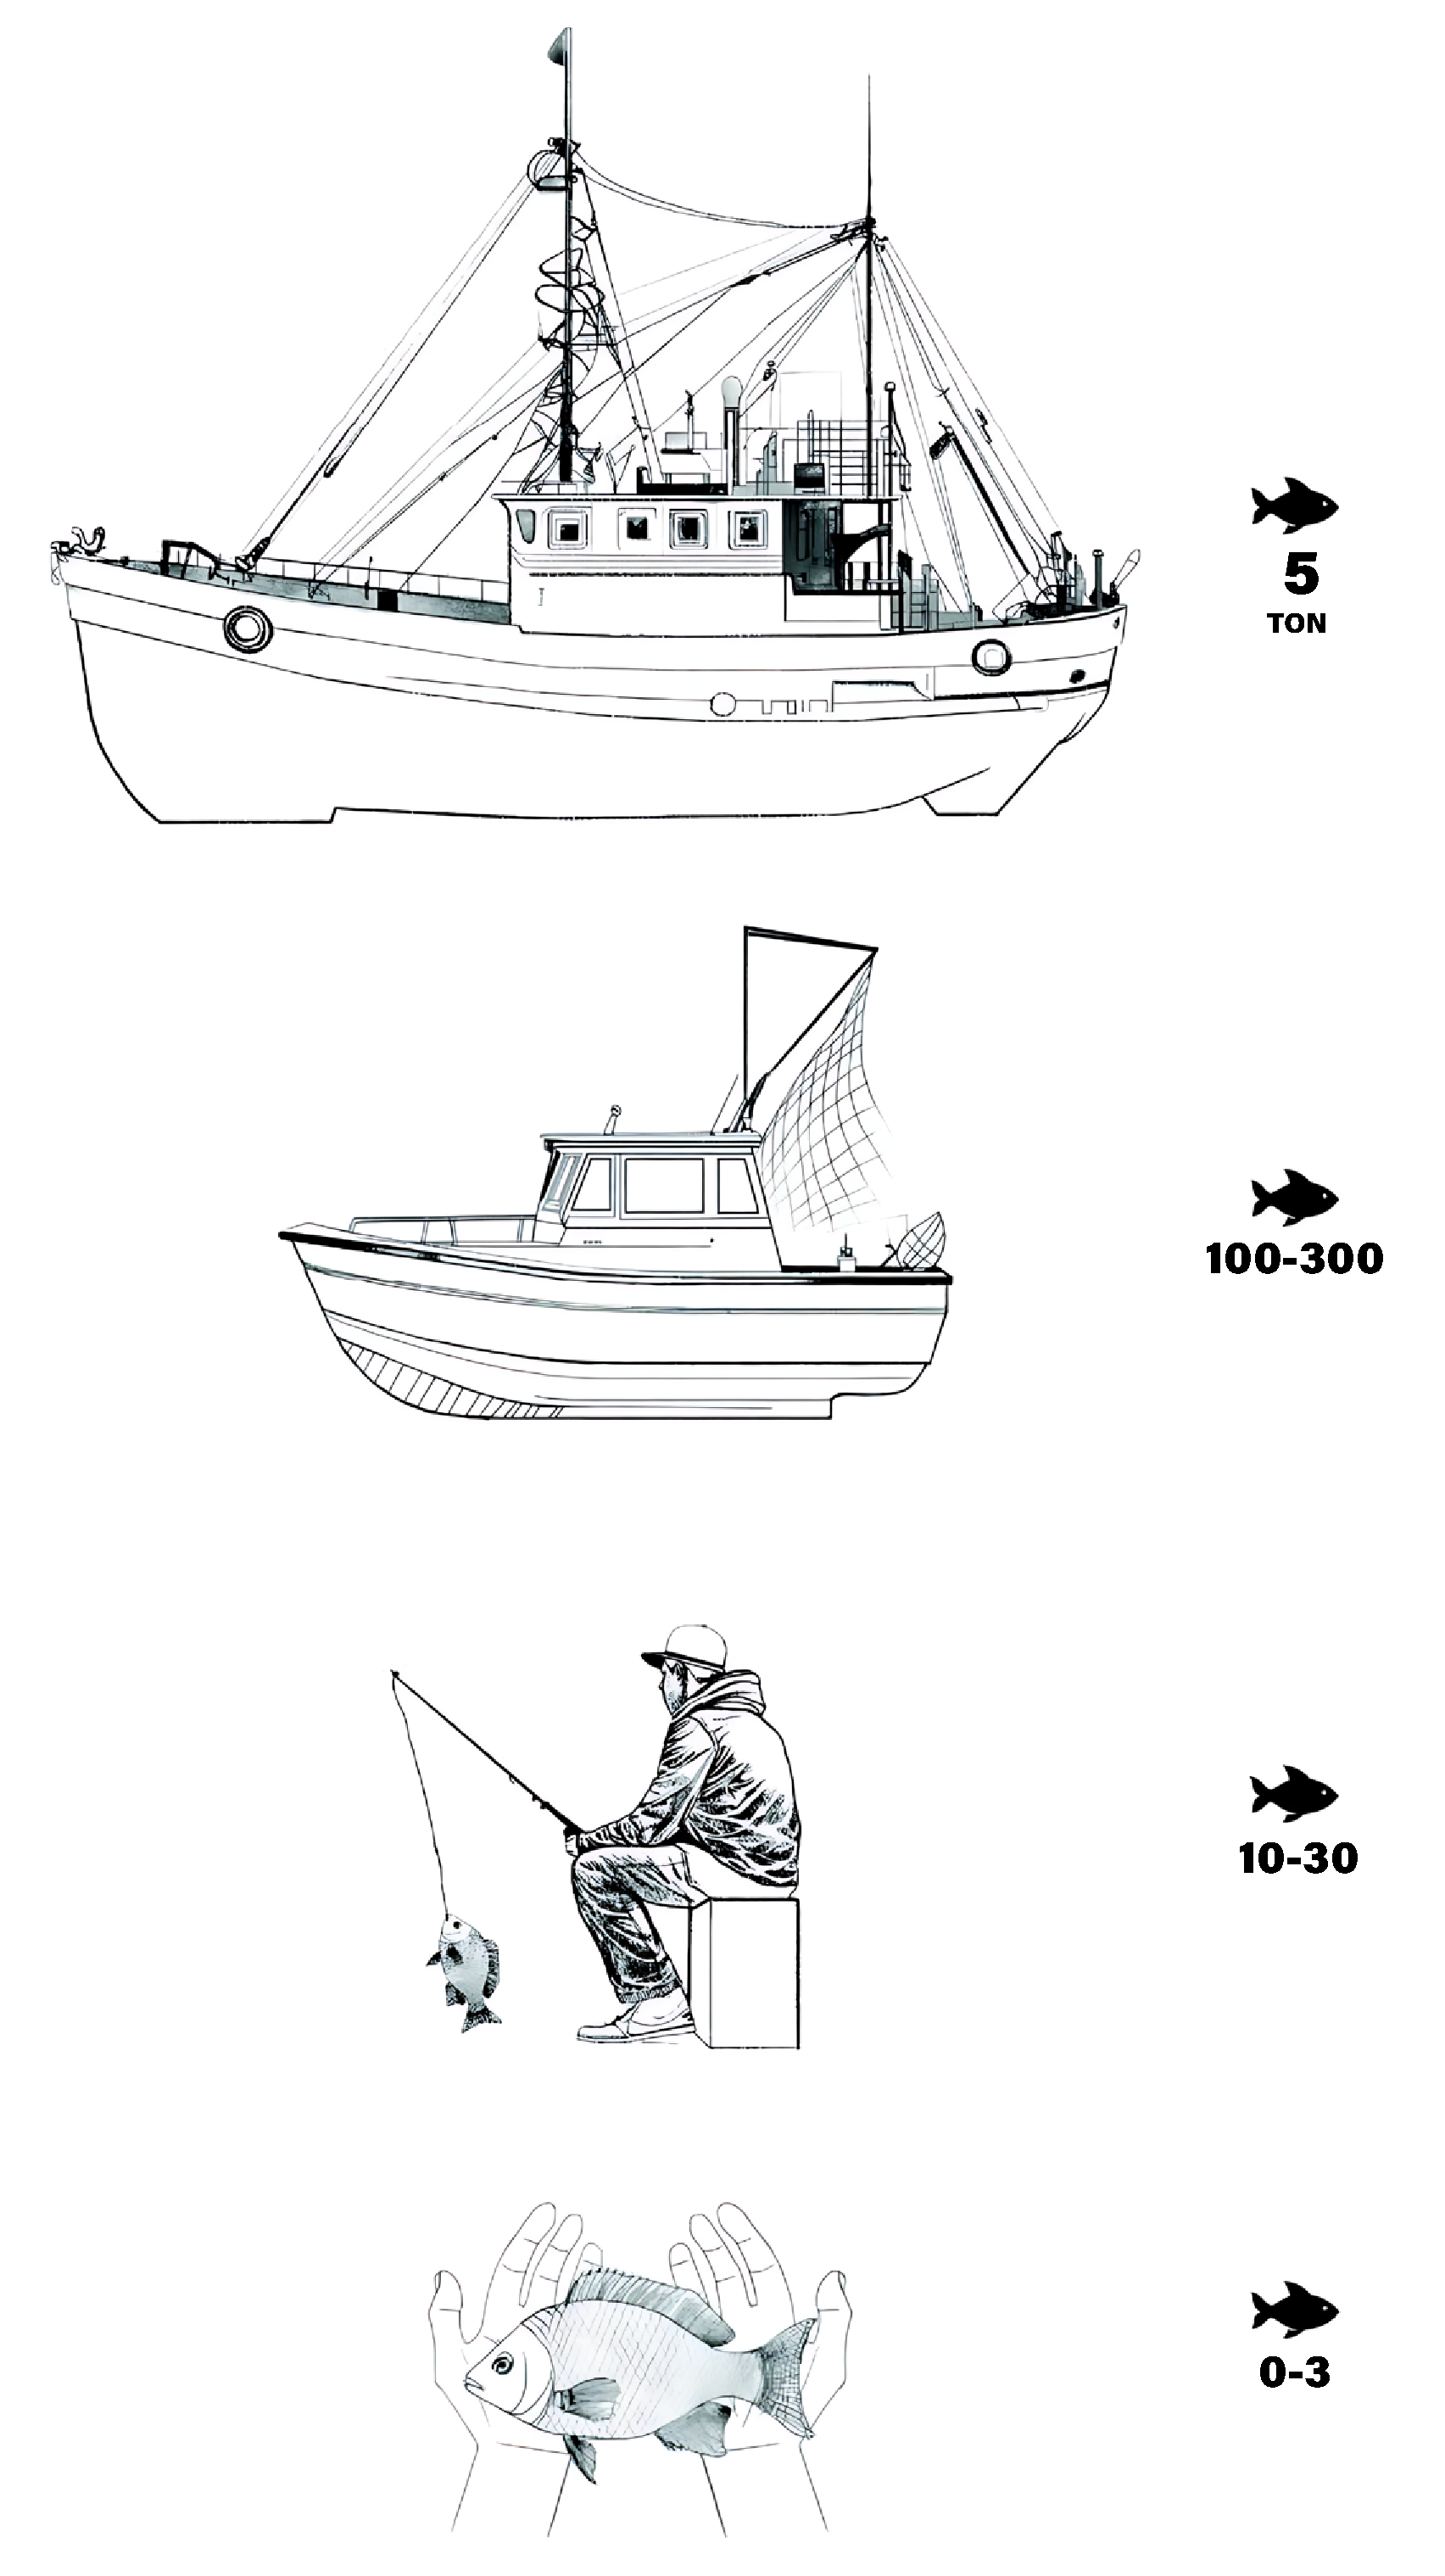
\includegraphics[width=0.8\textwidth]{figures/fig8.pdf}
    \caption[Productiviteit en kapitaal\index{kapitaal}]{Productiviteit en kapitaal\index{kapitaal}}
    \label{fig8}
\end{figure}

Deze toename in productiviteit is uiteindelijk wat het verschil in levensstandaard uitmaakt tussen mensen die met grote hoeveelheden kapitaal\index{kapitaal} kunnen werken en mensen die dat niet kunnen, tussen mensen die met hun blote handen vissen en mensen die met de Annelies Ilena vissen, tussen landen met een grote hoeveelheid industrieel kapitaal\index{kapitaal} en landen zonder.

Deze verhoogde productiviteit is wat ons moderne leven mogelijk maakt. Probeer als gedachte-experiment te overleven zonder gebruik te maken van enige kapitaalgoederen\index{kapitaalgoederen}. Als je alle productieprocessen met je blote handen zou moeten uitvoeren, dan zou overleven een zeer zware beproeving zijn. Het zou onzeker zijn of je door te hamsteren of te jagen genoeg voedsel zou kunnen vinden voor je dagelijkse overleving. Een schuilplaats die alleen met de hand gebouwd is, zou kwetsbaar zijn en gemakkelijk door de natuur kunnen worden vernietigd. Onder dergelijke omstandigheden zou overleven onzeker zijn. Maar als je zou overleven, is het bijna ondenkbaar dat je de enorme waarde van het investeren in de productie\index{productie} van goederen die de opbrengst van je tijd besteed aan productieprocessen verhogen, niet zou onderkennen. Het onvermijdelijke gebruik van stenen en takken voor het afweren van dieren of het jagen erop vormt op zich al een gebruik van kapitaal\index{kapitaal}. Individuen en ideologieën die de zogenaamde ``kwaden van kapitaal'' aan de kaak stellen, uiten hun onmacht en onwetendheid tegenover de onvermijdelijkheid dat het menselijke verstand gereedschappen inzet om zijn doelen te bereiken.

Als deze investeringen leiden tot een hogere productiviteit, dan wordt het veiligstellen van voedsel voor een dag minder belastend en minder onzeker. Er is minder tijd nodig voor het pure overleven, waardoor meer tijd overblijft om te investeren in verdere kapitaalproductie, met als doel de productiviteit nog verder te verhogen.

De meest zekere en belangrijkste manier om de levenskwaliteit van de mens te verhogen is door de accumulatie van kapitaalgoederen\index{kapitaalgoederen}, omdat deze dienen om de arbeidsproductiviteit te verhogen. Er is geen garantie dat investeren in kapitaal\index{kapitaal} zal leiden tot verhoogde productiviteit en dat is het inherente risico\index{risico} aan het proces van kapitaalaccumulatie. Maar als een investering kapitaal\index{kapitaal} oplevert dat niet leidt tot verhoogde productiviteit, dan mislukt de investering en de resultaten zullen niet als kapitaal\index{kapitaal} worden ingezet. Het zal geconsumeerd worden als dat mogelijk is, of anders afgedankt worden. Er zijn ongetwijfeld veel pogingen gedaan om kapitaalgoederen\index{kapitaalgoederen} te produceren die de productiviteit van de visserij verhogen, maar alleen de succesvolle zijn behouden gebleven. Alle andere zijn allang vergeten en de investeringen erin zijn verspild. Kapitaal is niet zomaar het product van elke investering in het verlengen van het productieproces\index{productieproces}. Kapitaal bestaat alleen uit de investeringen in het verlengen van het productieproces\index{productieproces} die hogere productiviteit opleveren. Het risico\index{risico} van verspilling is slechts één aspect van de hoge kosten van kapitaal\index{kapitaal}.

Hoe langer het productieproces\index{productieproces}, hoe meer kapitaal\index{kapitaal} succesvol wordt ingezet, hoe hoger de productiviteit van arbeid, hoe minder van de dagelijkse arbeid nodig is om puur te overleven, en hoe groter de veiligheidsmarge die de mens scheidt van verhongering. Het is voornamelijk dankzij het vergaren van kapitaal\index{kapitaal} en langere productieprocessen dat het merendeel van de wereldbevolking voedzaam eten kan kopen voor een fractie van een dagloon. Zonder modern kapitaal\index{kapitaal} zou de opbrengst van een dag werken ongeveer gelijk zijn aan wat een individu nodig heeft om een dag te overleven, wat het bestaan precair en onzeker zou maken. Extreme armoede bestaat tegenwoordig alleen nog op plekken waar kapitaal\index{kapitaal} schaars is en waar mensen de hele dag moeten werken om te overleven. Met modern kapitaal\index{kapitaal} daarentegen kunnen de meeste werknemers elke dag meerdere keren hun dagelijkse voedselbehoefte produceren, wat hen een aanzienlijke veiligheidsmarge biedt om hen te beschermen tegen armoede en hongersnood, en hen in staat stelt om vele andere goederen te consumeren.

Om het belang van kapitaal\index{kapitaal} te begrijpen, moet je proberen je werk te verrichten zonder enig kapitaal\index{kapitaal} en de verandering in je productiviteit te meten. Als je een boer bent, probeer dan je land te verbouwen met enkel je blote handen, zonder tractor of schop. Probeer te jagen zonder een geweer, speer, of pijl-en-boog. Probeer een taxichauffeur te zijn zonder auto. Probeer een winter te overleven zonder de kapitaalgoederen\index{kapitaalgoederen} die we gebruiken om onze moderne huizen te bouwen, ze te verwarmen en te beschermen tegen stormen. Het klopt om armoede te zien als gebrek aan kapitaal\index{kapitaal}.

Een goede literaire illustratie van de waarde van kapitaal\index{kapitaal} komt uit het werk \emph{Aan de Grond in Londen en Parijs} van George Orwell. \autocite{63} Orwell bracht veel tijd door met laagbetaalde arbeiders in beide grote Europese steden in de jaren `20 en `30. Een van zijn meest scherpzinnige en diepgaande observaties over de staat van armoede waarin hij leefde, was hoe duur alles was voor arme mensen. Een rijke man die een huis heeft met alle benodigdheden om te overleven, kan het van dag tot dag overleven als vanzelfsprekend beschouwen, althans in vergelijking met wat een arme zwerver moet doorstaan om in zijn basisbehoeften te voorzien. Zonder keuken is elke maaltijd duur. Zonder auto kost lopen veel tijd. Zonder kledingkast is het duur om fatsoenlijke kleren te vinden om er goed uit te zien voor een degelijke baan. Veel dingen worden goedkoper door het bezit van kapitaal\index{kapitaal}, en het gebrek aan kapitaal\index{kapitaal} is een belangrijke reden waarom armoede onoverkomelijk kan lijken. Lage voorraden van kapitaal\index{kapitaal} leiden tot lage productiviteit, wat op zijn beurt weinig ruimte overlaat voor sparen en investeren in kapitaal\index{kapitaal} om de productiviteit te verhogen. Het doorbreken van deze cyclus vereist het uitstellen van consumptie\index{consumptie} wanneer de consumptie\index{consumptie} al heel klein is, en overleven onzeker. Veel van \textquotesingle s werelds armen worstelen met het ontsnappen uit deze armoedecirkel.

\hypertarget{de-hoge-kosten-van-kapitaal}{%
\section{De hoge kosten van kapitaal}\label{de-hoge-kosten-van-kapitaal}}

Het is niet ongebruikelijk om in de mainstream media, academische kringen en andere bronnen van economisch analfabetisme, kapitaal\index{kapitaal} en de eigenaren ervan op een minachtende manier te horen bespreken. Kapitaal wordt vaak afgeschilderd als een instrument om arbeid uit te buiten, en de eigenaren ervan als de ontvangers van een oneerlijk voordeel ten koste van de rest van de samenleving. Zelden wordt er gesproken over de ware kosten en verantwoordelijkheden die gepaard gaan met het bezit van kapitaal\index{kapitaal}. Om kapitaal\index{kapitaal} te bezitten, moet je het eerst verdienen. Daarna moet je de consumptie\index{consumptie} ervan uitstellen door te sparen. Vervolgens moet je het effectief inzetten in de markt om een rendement te behalen dat groot genoeg is om het te behouden. De economische kosten van kapitaal\index{kapitaal} komen op verschillende manieren tot uiting:

\hypertarget{uitgestelde-voldoening}{%
\subsection{Uitgestelde voldoening}\label{uitgestelde-voldoening}}

\textbf{Het nadeel van kapitaalaccumulatie is dat het duur en onzeker is. Het vereist het opofferen van huidige consumptie\index{consumptie} om middelen te investeren die pas in de toekomst vruchten zullen afwerpen, en misschien helemaal geen vruchten zullen afwerpen}. Kapitaal vereist constant uitstel van beloning en consumptie\index{consumptie}. De opportuniteitskosten van kapitaal\index{kapitaal} zijn altijd misgelopen consumptie\index{consumptie}. Iedereen die enig kapitaal\index{kapitaal} bezit, kan dat op elk moment verkopen in ruil\index{ruil} voor consumptiegoederen\index{consumptiegoed}. Op het moment dat zijn hengel klaar is, kan de visser iemand vinden die hem een aanzienlijke hoeveelheid vis wil betalen in ruil\index{ruil} voor de hengel. Om te kunnen blijven produceren op het meer productieve niveau dat de hengel mogelijk maakt, moet de eigenaar elke dag de kans afwijzen om een hoeveelheid vis te accepteren in ruil\index{ruil} voor zijn hengel. Elke productieve machine ter wereld kan door haar eigenaar verkocht worden in ruil\index{ruil} voor consumptiegoederen\index{consumptiegoed} die hem direct voldoening geven. De eigenaren van de Annelies Ilena zouden in het komende jaar buitengewoon goed kunnen leven als ze het schip zouden verkopen en de opbrengsten ervan zouden uitgeven, maar ze blijven dat grandioze jaar opofferen ten gunste van het behoud van kapitaal\index{kapitaal} dat gedurende tientallen jaren in de toekomst inkomsten zal genereren.

Voordat enige kapitaalaccumulatie kan plaatsvinden, moeten individuen hun tijdsvoorkeur\index{tijdsvoorkeur} verlagen; ze moeten om voor de toekomst te kunnen zorgen hun toekomst hoger waarderen, wat ten koste gaat van het heden. Dit punt moet in gedachten worden gehouden wanneer economische analfabeten tekeer gaan tegen de eigenaren van kapitaal\index{kapitaal} omdat ze parasieten zouden zijn van de werknemers. De opoffering van huidige consumptie\index{consumptie} door deze eigenaren van kapitaal\index{kapitaal} in ruil\index{ruil} voor toekomstige beloning, is economisch\index{economisch} gezien niet anders dan de opoffering van vrije tijd door werknemers in ruil\index{ruil} voor toekomstige beloning. Als de eigenaren van kapitaal\index{kapitaal} daadwerkelijk niets zouden bijdragen aan het productieproces\index{productieproces}, dan zou hun consumptie\index{consumptie} van het kapitaalgoed\index{kapitaalgoederen}, in plaats van het aan de werknemers aan te bieden, geen verschil maken voor de productiviteit van de werknemers. Maar vraag elke willekeurige werknemer wat er met hun productiviteit zou gebeuren zonder kapitaal\index{kapitaal}, en de absurditeit van het haten van kapitaal\index{kapitaal} wordt duidelijk.

Het is de moeite waard om te vermelden dat noch de Marxistische noch de Keynesiaanse economische scholen van krom-denken ooit het intellectuele vermogen hebben ontwikkeld om met een concept als tijdsvoorkeur\index{tijdsvoorkeur} om te gaan en wat het voor kapitaalaccumulatie betekent. Evenmin hebben ze ooit begrip van het concept van opportuniteitskosten getoond, zoals blijkt uit hun beleidsvoorstellen, die passen in een Hof van Eden waar geen schaarste\index{schaarste} bestaat die regeringen of individuen dwingt keuzes te maken. Er is geen erkenning van de problematiek en het belang van kapitaalaccumulatie mogelijk zonder het begrip van schaarste\index{schaarste} en opportuniteitskosten, en dat helpt te verklaren waarom socialistische regeringen de algehele vernietiging van maatschappelijk kapitaal\index{kapitaal} bewerkstelligen.

\subsection{Vernietiging}

\textbf{Het produceren van kapitaal\index{kapitaal} is kostbaar en onzeker, en het vernietigen van kapitaal\index{kapitaal} is zeer gemakkelijk}. Kapitaal is vergelijkbaar met een levend organisme dat om te overleven voortdurend inputs moet ontvangen van, en outputs moet produceren voor zijn omgeving. Het moet opereren in een markt waar prijzen er de meest productieve toepassingen en productieprocessen voor bepalen. Prijzen informeren kapitalisten over waar ze hun kapitaal\index{kapitaal} moeten inzetten en ze verschaffen ondernemers informatie over hoe ze productieprocessen moeten beheren. Zonder vrije markten\index{markten} geven prijzen geen signalen aan kapitalisten of ondernemers over waar en hoe ze hun middelen moeten inzetten, wat leidt tot verkeerde allocatie en dus verspilling en een afname van kapitaalvoorraden. Zonder gebruik en goed onderhoud, raken machines defect en takelen ze af. Verstoringen van productieprocessen kunnen zeer kostbare en vaak onherstelbare schade aan kapitaalgoederen\index{kapitaalgoederen} veroorzaken. Onze visser heeft veel tijd nodig om zijn vissersboot te bouwen, maar het duurt slechts enkele seconden om de controle over de boot te verliezen, waardoor deze tegen een rotsachtige kust kan botsen en in onherstelbare stukken uiteen kan vallen. Dit geldt evenzeer voor de kleine vissersboot als voor de gigantische trawlers.

\subsection{Slijtage}

\textbf{Het is ook de aard van kapitaal\index{kapitaal} om in de loop van de tijd, naarmate het gebruikt wordt, in waarde te verminderen.} Kapitaal is niet eeuwig, en het dagelijks gebruik en slijtage eisen hun tol. Producenten die investeren in kapitaal\index{kapitaal} kunnen niet verwachten dat het oneindig blijft produceren op hetzelfde productiviteitsniveau. De productiviteit van kapitaal\index{kapitaal} neemt voortdurend af met gebruik en er zijn bijkomende kapitaaluitgaven nodig om kapitaal\index{kapitaal} te onderhouden en de productiviteit ervan te behouden. De kwaliteit van de visspeer gaat in het zoute zeewater achteruit en ze wordt minder effectief na verloop van tijd. Het kleine vissersbootje takelt met gebruik af en het vereist na verloop van tijd een investering van meer tijd om het te repareren. De meest geavanceerde moderne vissersboot heeft constant onderhoud nodig om in bedrijf\index{bedrijf} te blijven, en het beschikt over een groot team van gespecialiseerde ingenieurs en arbeiders die voortdurend de kritische onderdelen inspecteren, versleten onderdelen vervangen, de tandwielen smeren en de brandstof die het nodig heeft bijvullen.

\subsection{Risico}

Kapitaalaccumulatie is ook inherent risicovol en onzeker. Bovenop het risico\index{risico} van vernietiging dat hierboven is besproken, zijn er talloze redenen waarom kapitaal\index{kapitaal} mogelijk niet de gewenste kwaliteit en hoeveelheid eindproducten zou kunnen opleveren. Kapitaal loopt het risico\index{risico} om achterhaald te raken door de uitvinding van nieuwere producten en productiemethoden. Een ondernemer kan buiten haar eigen schuld ontdekken dat haar volledige investering achterhaald geraakt is, wanneer een concurrent een beter product ontwikkelt of een veel goedkopere manier om een product te maken. \textbf{Kapitaalaccumulatie vereist niet alleen het opofferen van het heden voor de toekomst, maar het vereist ook het opofferen van het zekere voor het onzekere.} De kapitalist speculeert constant dat haar investering in de toekomst een positief rendement zal opleveren, maar ze kan altijd verkeerd zitten.

Om kapitalist te worden, moet je eerst iets van waarde produceren waarvoor anderen kunnen betalen. De kapitalist moet dan afzien van het gebruik van die betaling voor eigen behoeften en deze in plaats daarvan in een bedrijf\index{bedrijf} steken met als doel anderen te dienen. Dit wordt bereikt door producten voort te brengen die de anderen subjectief hoger waarderen dan de marktprijs van de inputs in het productieproces\index{productieproces}. Op elk moment zal het het niet bieden van deze waarde aan klanten resulteren in het inzakken van omzet en winstgevendheid, wat onvermijdelijk leidt tot faillissement\index{faillissement} en het verlies van kapitaal\index{kapitaal}. De oorzaken van dergelijk falen zijn eindeloos: luiheid, desinteresse, pech, betere concurrenten, maar de uitkomst is altijd hetzelfde: het verlies van kapitaal\index{kapitaal}.

Dit zijn de redenen waarom kapitaalbezit zo waardevol en productief is, en waarom werknemers ervoor kiezen om voor eigenaren van kapitaal\index{kapitaal} te blijven werken. Zoals Murray Rothbard\index{Murray Rothbard} het verwoordde:

\begin{blockquotebox}
    Alle werknemers zouden kunnen weigeren om voor lonen te werken, zouden ze dat willen, en in plaats daarvan hun eigen productiecoöperaties vormen. Ze zouden jaren kunnen wachten om betaald te worden tot de producten aan de consumenten zijn verkocht. Het feit dat ze dit niet doen, toont het enorme voordeel van het systeem van kapitaalinvestering en loonbetaling. Dit systeem stelt werknemers in staat om ver voor de verkoop van hun producten geld te verdienen. In plaats van uitbuiting van de werknemers, is kapitaalinvestering en het systeem van winsten en rentes een enorme zegen voor hen en voor de hele samenleving. \footnotemark
\end{blockquotebox}
\footautocite{64}

\textbf{In een economisch\index{economisch} systeem van de vrije markt is de mate waarin een individu kapitaal\index{kapitaal} bezit gelijk aan de mate waarin hij mensen voldoende kan bedienen om zijn kapitaal\index{kapitaal} te behouden.} Er is geen privilege of erfenis die hierboven staat, noch een rijkdom te groot. Als je je klanten niet bedient, zal je kapitaal\index{kapitaal} in waarde afnemen tot het uiteindelijk nutteloze rommel wordt die moet worden afgedankt. Kapitaal bezitten, zo legde Mises uit, is een verantwoordelijkheid en een kwetsbaarheid, geen privilege.

\begin{blockquotebox}
    Kapitalisten en grondeigenaren moeten hun eigendom gebruiken voor de best mogelijke voldoening van de consumenten. Als ze hun verplichtingen traag en onbekwaam nakomen, worden ze afgestraft met verliezen. Als ze de les niet leren en hun gedrag niet verbeteren, verliezen ze hun rijkdom. Geen investering is voor altijd veilig. \footnotemark
\end{blockquotebox}
\footautocite{65}

Moderne economische scholen doceren de realiteit van economie niet als de studie van menselijk handelen\index{menselijk handelen}. Daardoor kunnen hun aanhangers het harde werk, de opoffering en risico\index{risico}\textquotesingle s die nodig zijn om eigenaar van kapitaal\index{kapitaal} te worden, niet begrijpen. Deze onmacht om oorzaak en gevolg te begrijpen leidt ertoe dat kapitaal\index{kapitaal} wordt voorgesteld als een soort hemels privilege dat aan een bepaald soort mensen wordt toegekend. Je behoort tot die soort of je behoort er niet toe. Er is weinig waardering of begrip voor de acties die nodig zijn om kapitaal\index{kapitaal} op te bouwen en het succesvol te behouden. Als gevolg hiervan verspillen veel mensen hun tijd en de vruchten van hun arbeid, door bitter te klagen over kapitaal\index{kapitaal} in plaats van te werken om het te verwerven en hun productiviteit en levensstandaard te verhogen. Deze economische onwetendheid is de wind in de zeilen van demagoog-politici die het uitbuiten om aan de macht te komen en deze te gebruiken om eigenaars van kapitaal\index{kapitaal} te onteigenen.

De minachting en het zwart maken van kapitaalbezit door Keynesianen en Marxisten en hun onvermogen om de noodzakelijke kosten voor kapitaalaccumulatie te begrijpen, heeft ertoe geleid dat regeringen onder invloed van deze ideologieën vaak hebben geprobeerd om investeringen te financieren zonder hiervoor te sparen. Of het nu gaat om het printen van fysiek geld of kredietexpansie, het onderliggende waanidee is hetzelfde: het creëren van claims op kapitaal\index{kapitaal} kan de noodzaak van sparen om kapitaal\index{kapitaal} te produceren vervangen. Deze dynamiek en haar rampzalige gevolgen zullen nader worden bestudeerd in Deel IV van dit boek.

\hypertarget{kapitaal-en-tijdsvoorkeur}{%
\section{Kapitaal en tijdsvoorkeur}\label{kapitaal-en-tijdsvoorkeur}}

\begin{blockquotebox}
    Een tijdsvoorkeur\index{tijdsvoorkeur} die laag genoeg is om sparen en kapitaalvorming of de productie\index{productie} van duurzame consumptiegoederen\index{consumptiegoed} mogelijk te maken, zet een neiging tot verdere daling ervan in gang. Dit gaat gepaard met een ``proces van beschaving\index{beschaving}''.\footnotemark
    \par\raggedleft--- Hans-Hermann Hoppe\index{Hans-Hermann Hoppe}
\end{blockquotebox}
\footautocite{66}

De kosten van kapitaalaccumulatie liggen in de opofferingen van huidige goederen om middelen te kunnen investeren in de productie\index{productie} van toekomstige goederen. Hoe hoger mensen het heden ten opzichte van de toekomst waarderen, oftewel hoe hoger hun tijdsvoorkeur\index{tijdsvoorkeur} is, hoe minder ze geneigd zullen zijn om consumptie\index{consumptie} uit te stellen en te investeren in toekomstige productie\index{productie}. Naarmate hun tijdsvoorkeur\index{tijdsvoorkeur} afneemt en hun waardering voor de toekomst toeneemt, zullen ze eerder afzien van huidige consumptie\index{consumptie} in een streven naar toekomstige rendementen. Voor zover bekend, kunnen kapitaalgoederen\index{kapitaalgoederen} niet uit het niets getoverd worden door verbeelding of wensdenken. De enige manier om kapitaalgoederen\index{kapitaalgoederen} te maken, ligt in het uitstel van de consumptie\index{consumptie} van huidige goederen. Zoals alle economische verschijnselen, kan kapitaal\index{kapitaal} alleen begrepen worden in termen van menselijk handelen\index{menselijk handelen} en de handelingen die nodig zijn om het te laten gebeuren. De beperking van kapitaalaccumulatie is niet iets natuurlijks of fysieks; ze is menselijk en het ligt er net aan hoeveel van hun productie\index{productie} mensen willen investeren in toekomstige productie\index{productie} versus huidige consumptie\index{consumptie}. \textbf{Met andere woorden, de beperkende factor op de productie\index{productie} van kapitaal\index{kapitaal} is de tijdsvoorkeur\index{tijdsvoorkeur}.} Zoals Hoppe uitlegde: ``Hoe lager de tijdsvoorkeur\index{tijdsvoorkeur}, hoe eerder het proces van kapitaalvorming begint en hoe sneller de productiestructuur grosso modo zal worden verlengd.'' \autocite{67}

Aangezien tijdsvoorkeur\index{tijdsvoorkeur} de beperkende factor op de productie\index{productie} van kapitaal\index{kapitaal} is, volgt daaruit dat de prijs\index{prijs} van kapitaal\index{kapitaal} een weerspiegeling van de tijdsvoorkeur\index{tijdsvoorkeur} is. Hoe lager iemands tijdsvoorkeur\index{tijdsvoorkeur}, hoe minder korting op de toekomst ten opzichte van het heden ze toepassen, en hoe goedkoper het is voor hen om de huidige consumptie\index{consumptie} op te offeren voor toekomstige beloning. Wanneer iemand echter een hoge tijdsvoorkeur\index{tijdsvoorkeur} heeft, zal het opofferen van huidige consumptie\index{consumptie} erg duur lijken in vergelijking met de toekomstige beloning. De prijs\index{prijs} van kapitaal\index{kapitaal} is dus een negatieve functie van de tijdsvoorkeur\index{tijdsvoorkeur}. Dit is de intuïtieve basis voor de zuivere theorie van rentes en tijdsvoorkeur\index{tijdsvoorkeur}, die in detail besproken wordt in Hoofdstuk IV van dit boek, na de introductie van geld, ondernemerschap en de monetaire economische marktorde in de komende hoofdstukken.

Aangezien tijdsvoorkeur\index{tijdsvoorkeur} positief is, stimuleert alleen de verwachting van een positief reëel rendement tot sparen. De waarde van kapitaalgoederen\index{kapitaalgoederen} wordt geheel afgeleid van de goederen die ze produceren; kapitaal\index{kapitaal} heeft geen waarde onafhankelijk van het product ervan omdat het mensen geen direct nut biedt als consumptiegoed\index{consumptiegoed}; het heeft alleen nut voor zover het goederen met gebruikswaarde kan produceren. Alleen investeringen in activiteiten die een positief rendement bieden qua nut en eindproducten, worden ondernomen. Zoals Rothbard stelde:

\begin{blockquotebox}
    We kunnen de gehele handeling van het beslissen of we een daad van kapitaalvorming wel of niet uitvoeren uitleggen als het afwegen van relatieve nuttigheden. Deze worden \textquotesingle verdisconteerd\textquotesingle{} door de tijdsvoorkeur\index{tijdsvoorkeur} van de beslisser en ook door de onzekerheidsfactor.\footnotemark
\end{blockquotebox}
\footautocite{68}

Wanneer iemand de toekomstige opbrengst van het productieproces\index{productieproces} hoger waardeert dan de benodigde initiële investering, rekening houdend met zijn tijdsvoorkeur\index{tijdsvoorkeur} en onzekerheid, is hij geneigd om te investeren en kapitaalgoederen\index{kapitaalgoederen} te produceren of aan te schaffen. Mocht de investering slagen, dan kan hij meer van de middelen gebruiken om meer kapitaalgoederen\index{kapitaalgoederen} te verwerven, waardoor zijn winsten en productiviteit verder toenemen. Naarmate de voorraad aan kapitaal\index{kapitaal} en productiviteit in de loop van de tijd toeneemt, wordt hij minder onzeker over zijn financiële toekomst. Dit verlaagt zijn tijdsvoorkeur\index{tijdsvoorkeur} verder, wat meer kapitaalaccumulatie aanmoedigt. Naarmate er in de samenleving meer kapitaal\index{kapitaal} wordt opgebouwd en de tijdsvoorkeur\index{tijdsvoorkeur} afneemt, daalt ook de prijs\index{prijs} van kapitaal\index{kapitaal} (die wordt bepaald door de rente\index{rente}). Dit proces van het verlagen van tijdsvoorkeur\index{tijdsvoorkeur} en toenemende investeringen kan begrepen worden als het proces van beschaving\index{beschaving}.

\hypertarget{misvattingen-over-sparen}{%
\section{Misvattingen over sparen}\label{misvattingen-over-sparen}}

Moderne economische leerboeken besteden weinig aandacht aan het proces van kapitaalaccumulatie. Wanneer mensen aan een kapitalistisch systeem denken, denken ze eerder aan vrijhandel als het kenmerkende onderdeel dan aan kapitaalaccumulatie. Internationale ontwikkelingsorganisaties die economische groei in ontwikkelingslanden bevorderen, benadrukken ook de rol van handel en talloze hervormingen van handelsbeleid, maar hechten weinig waarde aan kapitaalaccumulatie. Voor zover er sprake is van kapitaalaccumulatie, wordt het gebruikt als voorwendsel om publieke en private leningen te rechtvaardigen, alsof dat het equivalent zou zijn van het accumuleren van kapitaal\index{kapitaal}, terwijl het in feite precies het tegenovergestelde is. Internationale financiële instellingen zijn belanghebbende bij het genereren van meer leningen voor ontwikkelingslanden, maar hebben niet veel belangstelling voor de groei van binnenlandse spaartegoeden\index{spaartegoeden}.\autocite{69}

In moderne economische leerboeken wordt heel weinig gesproken over sparen, vooral als het gaat om de essentiële rol van sparen bij het genereren van economische productie\index{productie}. Het sparen in financiële instrumenten, in plaats van ze uit te geven, verschilt niet van het sparen van economische middelen van de huidige consumptie\index{consumptie} om ze in te zetten voor economische productie\index{productie}, of van het uitstellen van het genot van vrije tijd om arbeid te verrichten. Ook de onontkoombare noodzaak van sparen voorafgaand aan investeren wordt niet besproken. In plaats van de gemeenschappelijke factor van het uitstellen van beloning in al deze handelingen te benadrukken, en hun onmisbare rol in economische groei en vooruitgang, portretteert het typische Keynesiaanse leerboek sparen als een asociale en bijna sociopathische persoonlijkheidsstoornis.

Het startpunt van de Keynesiaanse analyse is de veronderstelling dat het inkomen van de samenleving wordt verdeeld in uitgaven en sparen volgens een vooraf bepaalde wiskundige formule. Er is weinig discussie over de factoren die het spaarniveau in een samenleving bepalen. Het belang van menselijk handelen\index{menselijk handelen} bij het maken van deze keuze wordt niet onderkend en er wordt niet over de gevolgen ervan gesproken. Het Keynesiaanse model gebruikt een zeer gekunstelde definitie van sparen waarvan de uitleg en weerlegging niet meer dan een voetnoot in dit boek verdienen.~\footnote{Dit is hoe Mankiw's Principles of Economics sparen en investeringen uitlegt. Het identificeren van de vele categoriefouten die nodig zijn om het Keynesiaanse stelsel van vergelijkingen werkbaar te maken, is een oefening voor de lezer: ``De termen sparen en investeren kunnen soms verwarrend zijn. De meeste mensen gebruiken deze termen terloops en soms door elkaar. De macro-economen die de nationale rekeningen samenstellen, gebruiken deze termen daarentegen zorgvuldig en duidelijk.''

\hspace{1em}``Bijvoorbeeld. Stel dat Larry meer verdient dan hij uitgeeft en zijn onuitgegeven inkomen bij een bank\index{bank} stort of gebruikt om aandelen of obligaties van een bedrijf\index{bedrijf} te kopen. Omdat Larry\textquotesingle s inkomen hoger is dan zijn consumptie\index{consumptie}, draagt hij bij aan het nationale sparen. Larry denkt misschien dat hij zijn geld ``investeert'', maar een macro-econoom zou Larry\textquotesingle s handeling eerder sparen noemen dan investeren. In de taal van de macro-economie verwijst investeren naar de aankoop van nieuw kapitaal\index{kapitaal}, zoals machines of gebouwen. Als Moe van de bank\index{bank} leent om een nieuw huis te bouwen, draagt hij bij aan de investering van het land. (Denk eraan, de aankoop van een nieuw huis is de enige vorm van huishoudelijke uitgaven die een investering is in plaats van consumptie\index{consumptie}). Op dezelfde manier draagt de Curly Corporation ook bij aan de investeringen van het land wanneer ze wat aandelen verkoopt en de opbrengst gebruikt om een nieuwe fabriek te bouwen.''

\hspace{1em}``Hoewel de boekhoudkundige identiteit S = I laat zien dat sparen en investeren gelijk zijn voor de economie als geheel, hoeft dit niet waar te zijn voor elk individueel huishouden of bedrijf\index{bedrijf}. Larry\textquotesingle s spaargeld kan meer zijn dan zijn investeringen, en hij kan het overschot op een bank\index{bank} zetten. Moe\textquotesingle s spaargeld kan minder zijn dan zijn investeringen en het tekort kan hij lenen bij een bank\index{bank}. Banken en andere financiële instellingen maken deze individuele verschillen tussen sparen en investeringen mogelijk door toe te staan dat het sparen van de een de investering van de ander financiert.''}

Het volstaat te zeggen dat de Keynesiaanse analyse na uitgebreide definitie- en wiskundige trucs concludeert dat evenwicht alleen wordt bereikt wanneer de hoeveelheid spaargelden gelijk is aan de hoeveelheid investeringen, ondanks het feit dat dit twee volledig verschillende concepten en boekhoudkundige posten zijn, en er geen reden is voor hen om gelijk te zijn, behalve door toeval. Maar volgens dit model betekent het, dat wanneer het totale sparen groter is dan de totale investeringen, dat de samenleving niet genoeg consumeert, of met andere woorden, te veel spaart. Het Keynesiaanse model stelt dat wanneer mensen besluiten om niet veel uit te geven en in plaats daarvan te sparen en geld op te potten, de economie afkoelt, wat leidt tot wijdverspreide werkloosheid en faillissementen.

Keynesiaanse leerboeken beschuldigen sparen van het schaden van de economische orde en het veroorzaken van werkloosheid. Ze doen dit op basis van respect voor Keynes\textquotesingle{} autoriteit en door meer recente ongeldige wiskundige vergelijkingen en modellen te gebruiken. Er wordt ook geconcludeerd dat sparen de markt zou beletten te herstellen, omdat de economie in een deflatoire spiraal terechtkomt, met minder uitgaven die leiden tot minder werkgelegenheid, wat op zijn beurt weer leidt tot minder uitgaven in een oneindige neerwaartse spiraal. Zo\textquotesingle n absurd scenario is begrijpelijk, omdat Keynes geen begrip had van hoe prijzen functioneren en zich aanpassen in een markteconomie, waar eindproducten afgeprijsd en uitverkocht worden, en onrendabele productiefactoren ingezet worden in nieuwe, meer productieve productielijnen. Maar volgens Keynes zouden markten\index{markten} er niet in slagen om zich aan te passen wanneer mensen egoïstisch hun eigen belang voorop stellen door te sparen, in plaats van het verantwoordelijke te doen en uit te geven.

Volgens Keynesianen kon alleen de almachtige en alwetende hand van dwingende overheidsinterventie de markt redden van de ramp die spaarders met een lage tijdsvoorkeur\index{lage tijdsvoorkeur} hadden veroorzaakt door in hun toekomst te voorzien ten koste van het heden. Door de spaargelden van de vrekken te devalueren om kredietgroei en overheidsuitgaven te financieren, zou de overheid\index{overheid} tegelijkertijd het totaalniveau van de uitgaven in de samenleving kunnen verhogen, de hoeveelheid investeringen kunnen laten toenemen, het spaargeld laten afnemen en voor alle zekerheid de spaarders een lesje zou leren en een voorbeeld zou stellen dat hen ontmoedigt om in de toekomst nog te sparen. Het uitgangspunt is dat door centrale planning alles mogelijk is. Dit was immers de doctrine van een man wiens tijdsvoorkeur\index{tijdsvoorkeur} zo hoog was en die zo weinig om de toekomst gaf dat hij het tot zijn motto maakte: ``Op de lange termijn zijn we allemaal dood.'' Gezien het feit dat sparen een manier is om voor de toekomst te voorzien, heeft Keynes nooit nagelaten het te kleineren, te ontmoedigen en te ondermijnen, en in dit opzicht is zijn economische theorie in overeenstemming met zijn persoonlijke moraal, zoals besproken wordt in Hoofdstuk 18.

De triomf van de Keynesiaanse economische theorie in moderne universiteiten weerspiegelt zich in de vernietiging van sparen en de cultuur eromheen. De westerse samenlevingen die de Industriële Revolutie en de voordelen van het moderne kapitalisme\index{kapitalisme} hebben meegemaakt dankzij vele decennia van sparen en kapitaalaccumulatie, hebben momenteel lage spaarpercentages. Deze percentages zijn al tientallen jaren op dit niveau. Het inflatoir monetair beleid, dat door Keynesianen wordt aangeprezen als de motor van economische groei, ontmoedigt mensen om te sparen. Wanneer deze inflatie\index{inflatie} resulteert in de onvermijdelijke crises, die in latere hoofdstukken van het boek worden besproken, geven de Keynesianen de schuld aan het sparen, en stellen meer inflatie\index{inflatie} voor om de gevolgen van inflatie\index{inflatie} te verhelpen.

\hypertarget{beperkingen-aan-kapitaal}{%
\section{Beperkingen aan kapitaal}\label{beperkingen-aan-kapitaal}}

Naarmate hoeveelheden kapitaal\index{kapitaal} tot voorbij een bepaald punt zijn opgebouwd terwijl andere factoren constant blijven, neemt de marginale productiviteit van kapitaal\index{kapitaal} af. Een textielfabriek die machines voor zijn arbeiders aanschaft, zal een zeer snelle productiviteitsgroei ervaren met de eerste machine die het koopt. De productiviteit neemt toe met elke arbeider die overstapt van werken met zijn handen naar het gebruik van een naaimachine. Elke extra machine zal echter een kleiner marginaal voordeel opleveren dan de voorgaande machines. De extra machine zal bijvoorbeeld gebruikt worden als reserve voor als een van de andere machines kapot gaat, dus de marginale bijdrage zal lager zijn dan die van de voorgaande machine die continu werd gebruikt. Naarmate er meer machines aangeschaft worden zonder overeenkomstige toename van arbeidskrachten en andere productiefactoren, en zonder technologische verbetering, neemt de marginale productiviteit van elke eenheid af. Het overstappen van handmatig vissen naar het gebruik van een hengel verhoogt de productiviteit van de visser meer dan het overstappen van één hengel naar twee.

Deze relatie heeft sommige economen tot de hypothese gebracht dat er grenzen zijn aan kapitaalaccumulatie, of dat kapitaalaccumulatie de economische groei op de lange termijn niet kan opstuwen. Hoewel dit strikt genomen waar is in een wereld waarin kapitaal\index{kapitaal} groeit terwijl andere productiefactoren ongewijzigd blijven, illustreert een vluchtige blik op de echte wereld om ons heen hoe ver dit van de realiteit afstaat. In de echte wereld heeft de accumulatie van kapitaal\index{kapitaal} geen afnemende marginale opbrengst omdat technologische kennis voortdurend groeit, waardoor we niet alleen meer, maar ook beter kapitaal\index{kapitaal} kunnen accumuleren. Technologische vooruitgang is \emph{zélf} een functie van toenemende kapitaalaccumulatie. Met andere woorden, hoe meer kapitaal\index{kapitaal} beschikbaar is, hoe meer technologieën uitgeprobeerd kunnen worden en hoe meer technologieën uitgevonden zullen worden. De beschikbaarheid van kapitaal\index{kapitaal} is de noodzakelijke voorwaarde om de productiestructuur te verlengen en nieuwe technologieën te introduceren. Ideeën voor technologieën zijn vrij goedkoop, maar de toepassing ervan is duur omdat er kapitaal\index{kapitaal} voor nodig is, wat duur is.

In de echte wereld blijft een visser niet investeren in het accumuleren van een steeds groter aantal hengels met afnemende marginale productiviteit. In plaats daarvan zal hij investeren in andere, meer productieve technologieën, zoals een visnet, een vissersboot en uiteindelijk, de Annelies Ilena. Hoewel het lijkt alsof we te veel kapitaal\index{kapitaal} kunnen hebben, is er in de praktijk, zolang er nog een visser is die minder productief is dan de Annelies Ilena, nog steeds veel ruimte voor kapitaalaccumulatie in de visindustrie, zelfs zonder enige nieuwe innovatie.

Zelfs de Annelies Ilena kan niet beschouwd worden als het toppunt van kapitaalproductiviteit in de visindustrie. Er is niets in dit schip dat het tot het hoogst mogelijke productiviteitsniveau voor visserij maakt. Een kapitalist met meer middelen zou opdracht kunnen geven tot de bouw van een nog productievere boot, met een nog langer productieproces\index{productieproces} voor het ontwerpen, bouwen en varen. Meer motoren zouden de snelheid kunnen verhogen, grotere vriezers zouden de opslagcapaciteit kunnen vergroten, meer netten zouden de vangstcapaciteit kunnen vergroten. Als kapitaal\index{kapitaal} en tijd ter beschikking worden gesteld aan de beste en meest ervaren scheepsingenieurs ter wereld, is het zeer onwaarschijnlijk dat ze geen productievere boot zouden kunnen ontwerpen dan de Annelies Ilena. De reden waarom we geen boot hebben die productiever is dan de Annelies Ilena is simpelweg dat we niet meer kapitaal\index{kapitaal} hebben geïnvesteerd in de bouw van vissersboten, waarvan de kapitaalaccumulatie wordt beperkt door ons vermogen om te sparen en onze tijdsvoorkeur\index{tijdsvoorkeur}. Het is niet zo dat we het einde van de kapitaalaccumulatie hebben bereikt, noch dat we zonder ideeën zitten om de vissersboten van nu te verbeteren.

De limiet op kapitaalinvesteringen bestaan uit de huidige opportuniteitskosten uitgedrukt in huidige goederen. De opportuniteitskosten van kapitaal\index{kapitaal} kunnen nooit zo laag worden dat we daardoor met te veel kapitaal\index{kapitaal} zouden komen te zitten. De reden dat er geen productievere boot dan de Annelies Ilena is gebouwd, is dat potentiële investeerders meer waarde hechten aan andere investeringsmogelijkheden of consumptie\index{consumptie} dan dat ze het risico\index{risico} nemen voor de productie\index{productie} van deze grotere boten.

Hoe meer kapitaal\index{kapitaal} we vergaren, hoe hoger de productiviteit van onze tijd, hoe meer we onze tijd waarderen, des te hoger de waarde van vrije tijd en daardoor hoe duurder het is om vrije tijd op te offeren voor arbeid en kapitaal\index{kapitaal}. Na verloop van tijd en met verdere kapitaalaccumulatie zullen er nieuwere en betere boten gemaakt worden. Meer geavanceerde trawlers nemen niet zomaar de vis af van de vissers met minder geavanceerde apparatuur. In plaats daarvan stellen ze vissers in staat om dieper te vissen, vis te vinden die door de andere vissers helemaal niet gevangen zou zijn, en zo meer vis naar de markt te brengen, waarmee aan de behoeften van meer consumenten wordt voldaan.
